\documentclass[conference]{IEEEtran}
\IEEEoverridecommandlockouts
% The preceding line is only needed to identify funding in the first footnote. If that is unneeded, please comment it out.
\usepackage{cite}
\usepackage{amsmath,amssymb,amsfonts}
\usepackage{algorithmic}
\usepackage{graphicx}
\usepackage{textcomp}
\usepackage{xcolor}
\def\BibTeX{{\rm B\kern-.05em{\sc i\kern-.025em b}\kern-.08em
    T\kern-.1667em\lower.7ex\hbox{E}\kern-.125emX}}
\begin{document}

\title{IEEE PAPER ON TRANSCRIBO*\\
{\footnotesize \textsuperscript{*}Note: Transcribo is in alpha phase and should not be considered a viable option for industry deployment}
\thanks{COEP Tech University .}
}

\author{\IEEEauthorblockN{Avdhut Kamble}
\IEEEauthorblockA{\textit{Computer Engineering, College of Engineering, Pune} \\
\textit{SPPU, Autonomous}\\
Pune, India \\
avdhut.kamble776@gmail.com}
\and
\IEEEauthorblockN{Meerali Naseet}
\IEEEauthorblockA{\textit{Computer Engineering, College of Engineering, Pune} \\
\textit{SPPU, Autonomous}\\
Pune, India \\
meerali.n@gmail.com}

% \IEEEauthorblockN{Dilip Kulkarni}
% \IEEEauthorblockA{\textit{Computer Engineering, College of Engineering, Pune} \\
% \textit{SPPU, Autonomous}\\
% Pune, India \\
% dilip.kulkarni@gmail.com}
% \and
% \IEEEauthorblockN{Shweta Kulkarni}
% \IEEEauthorblockA{\textit{Computer Engineering, College of Engineering, Pune} \\
% \textit{SPPU, Autonomous}\\
% Pune, India \\
% shweta.kulkarni@gmail.com}
 }

\maketitle

\begin{abstract}
Due to the Pandemic, the majority of Businesses and Educational institutes have switched over to online teaching and online meetings. Due to Network issues, device compatibility and server-side problems the students attending online classes are affected very badly, moreover the business meetings are also not attended by many professionals, and due to this they face many problems.
‘Transcribo’ project is created to solve this problem. It transcribes the Online video lectures/meetings to produce their summary/report resp., and also adds the highlights/topics to the content present, with features which add to the productivity of the peoples working online!
This project was created during the Codebreak2.0 Hackathon, using Python as a Backend Language and HTML \& CSS is used for Frontend Development. 

\end{abstract}

\begin{IEEEkeywords}
component, formatting, style, styling, insert
\end{IEEEkeywords}

\section{Introduction}
      
The project ‘Transcribo’ was developed during CodeBreak 2.0 Hackathon, which was conducted online.
This project is developed to solve and reduce the problems to some extent, faced by the students and all online medium users during Meetings or online teachings.
With the help of this project anyone can get the transcribed file which is not limited to summary only, but also highlights the main key points of the long transcription.
It uses the audio or video format file as an input and produces the transcript file as an output. For further, clarity and wider applicability and use we have given it a form of a Web application, so that it doesn’t get a limited to computer or Mobile users.

\section{Literature Review}

\subsection{Maintaining the Integrity of the Specifications}

According to JC Richards and T.S. Rogers (2014), CLIL and CBI are built around the core principles, one of which states that people learn a second language more succesfully when they use the language as a means of understanding content rather than language alone. It was cited by K. Elwood (2018) that CBI is an earlier model of CLIL And the term CBI and CLIL are interchangeably used in this paper. The findings of the study are presented in the subsequent section. Afterwards, the findings are discussed in light of relevant literature. Some concluding remarks are provided at the cod of the paper.~\cite{GNU}

\section{Applications}

This project has wide range of applications, some of which are listed below:-
For School/College Students, to get notes, if they missed any class by chance.
For School/College Students, to get notes with highlighted keywords, to revise the class during examinations.
For Business professionals to get the minutes of meeting.
For all the online events and workshops, which happens online, and after that report is to be prepared.
To know the name of medicines and brief of call, when the doctor consults the patients online using video/audio call. 
To store the financial based startup’s (like policy bazaar) call data in transcripted files, for future evidence and reference.
For all Specially abled who can’t hear the audio/video can see the transcription.~\cite{NLP}
+
	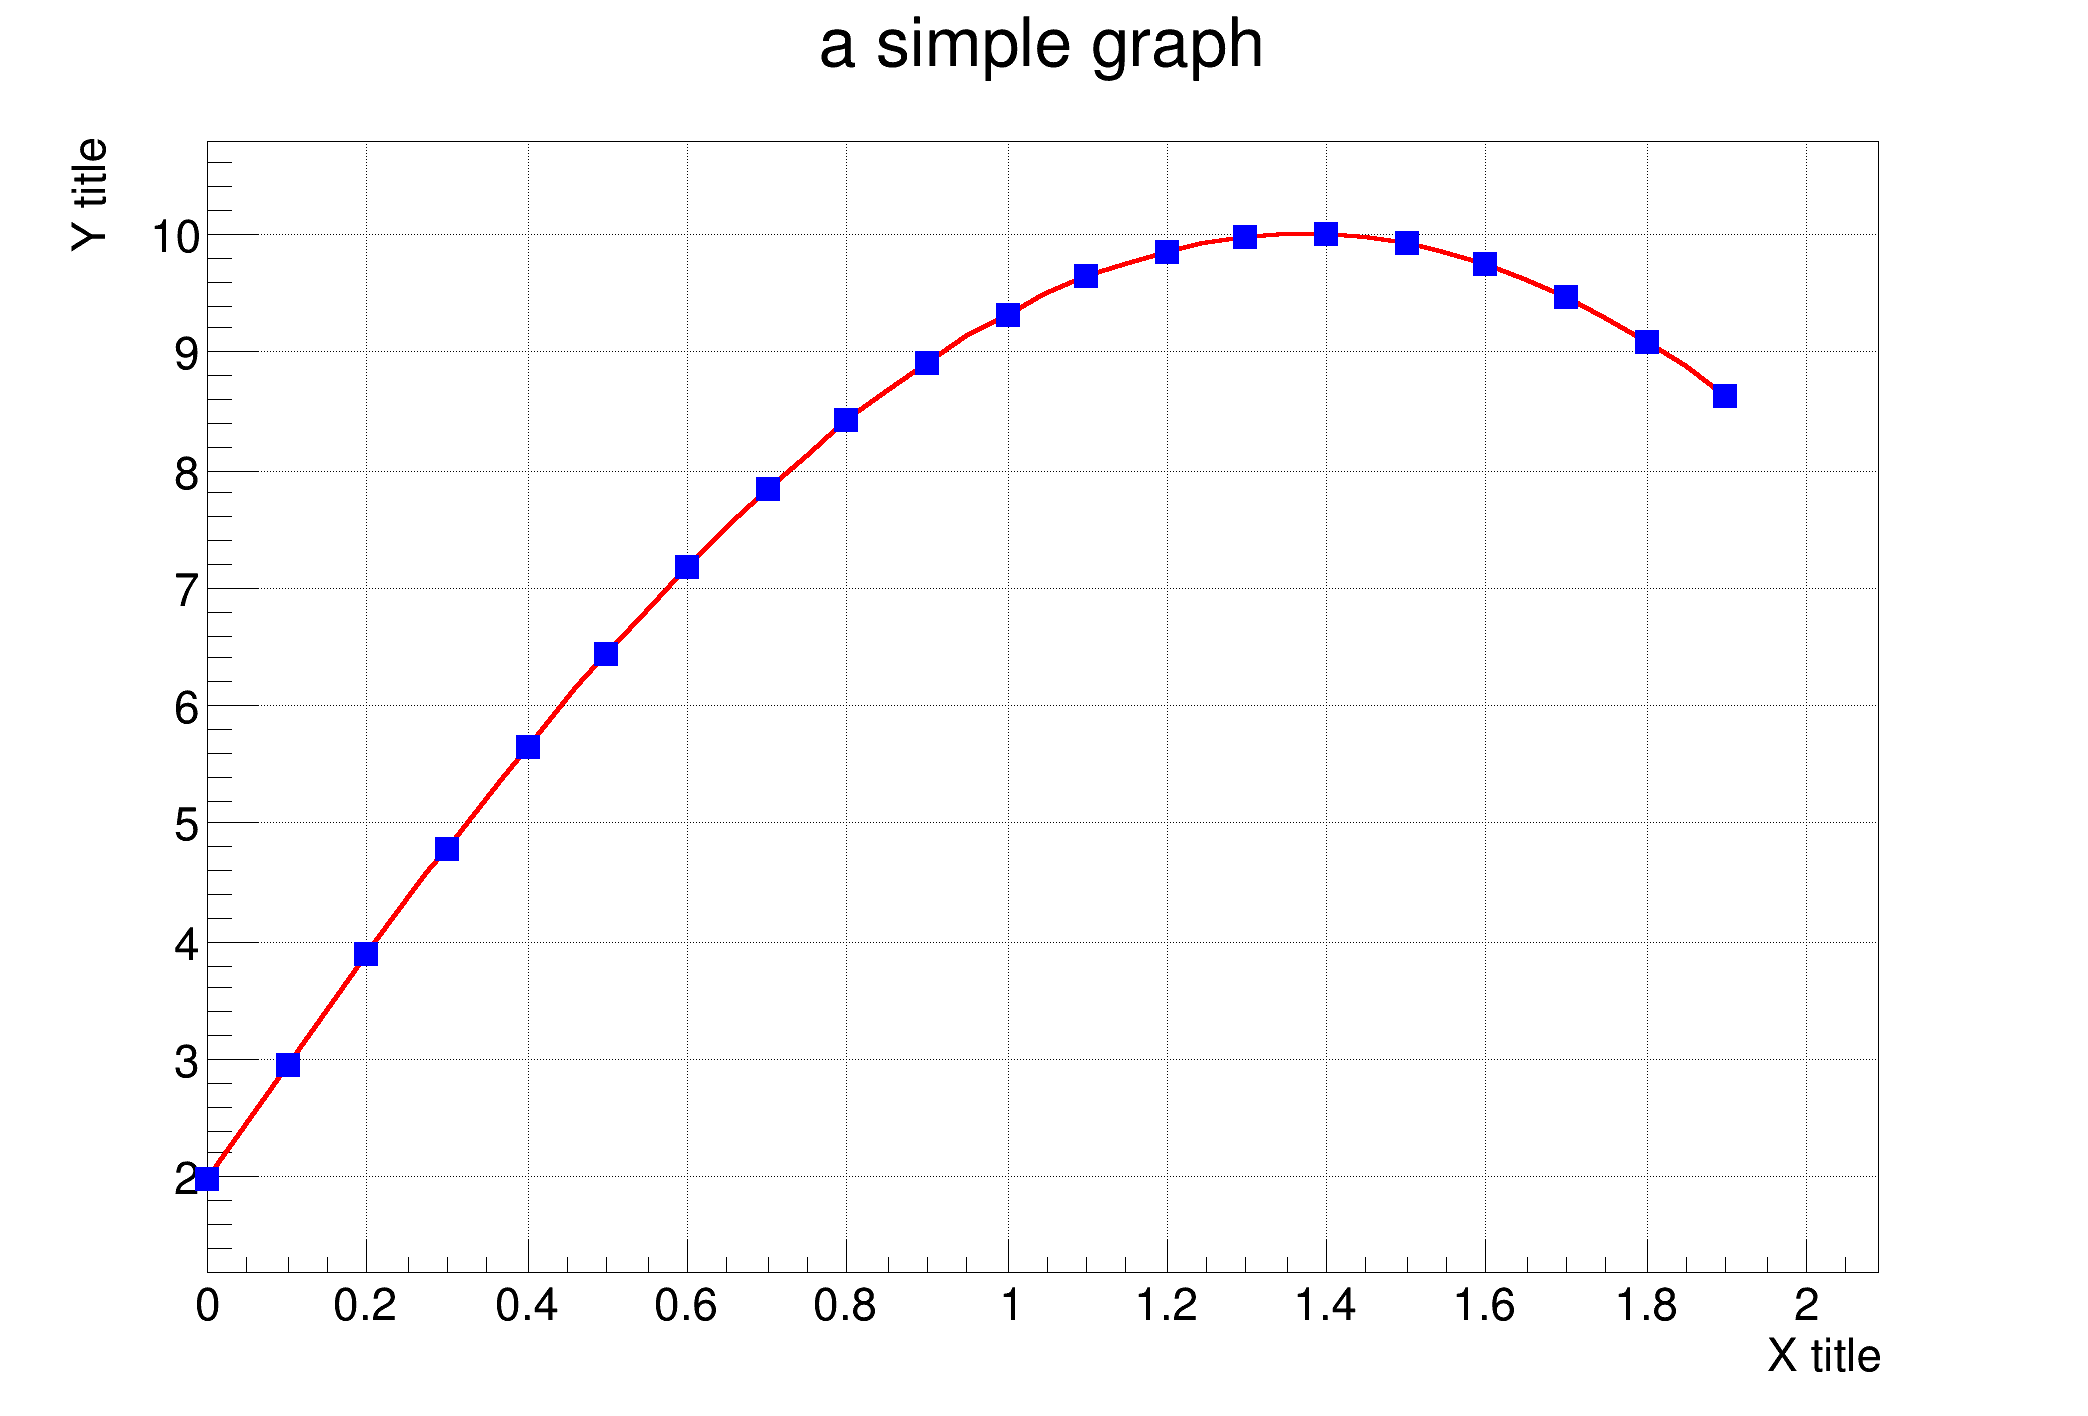
\includegraphics[height=6cm]{graph.png}


\section*{Conclusion and Future scope}

This project has many applications and benefits to humans across the globe with its specially designed features and platform independent service, as it is a web application.
The future of the world is Digital in nature, and this project can prove to be the one of the most important and needed to all the users who are digitally connected to the virtual world, while providing virtual services, can use it without any technical knowledge, due to its simple and easy to use operating features.



	\begin{thebibliography} {}
	
	\bibitem {NLP}Neil Deyw Stallman.,https://www.NLP.com/training-tutorials/linus-torvalds-and-richard-stallman/
	
	\bibitem{Wikipedia}JavaTpoint , https://www.javatpoint.com/nlp
	
	\bibitem{GNU} Richard Stallman, Linus Torvalds https://www.gnu.org/gnu/linux-and-gnu.en.html
	
		\end{thebibliography}
	

\end{document}
